\section{3-COLORING\footnote{%
Exercise 7.29 from the reference book: Sipser M.,
\emph{Introduction to the Theory of Computation}, 3rd edition (2013).
In the second edition of the book, this exercise is Exercise 7.27.}}

\subsection{Introduction}

Let us recall the big picture. We have shown in the first part of the course,
the part about computability, that not all problems can be solved by means of
Turing machines. We made the distinction between decidable and undecidable
problems, the former being the ones we can solve with algorithms, that is,
procedures that eventually terminate.

The second part, that is, the part about complexity, focuses on the resources
it takes to solve decidable problems. We already introduced the classes P and
NP\@. NP is the class of problems for which there exists a nondeterministic
polynomial-time algorithm. An equivalent definition is to consider the
languages for which all words have at least one corresponding membership
certificate of polynomial size that can be verified using a polynomial-time
algorithm called a verifier. P is the class of problems for which there exists
a deterministic polynomial-time algorithm, that is, algorithms we consider
efficient. By definition P is contained in NP\@.
However, we do not know whether P is different from NP, that is, whether
deciding is as easy as verifying, or, equivalentely, whether deterministic
algorithms are as powerful as nondeterministic ones.

Later on in the lectures, we will define the notion of NP-completeness and show
that, while we (today) cannot answer the question ``P vs. NP'', we can identify
a set of problems, the NP-complete problems, that capture the complexity of all
the problems in NP\@. This kind of result relies heavily on the notion of
reduction.

\subsection{Definitions}

We already saw that the reducibility of a problem to
another need not rely on similarity between the two problems. It is
possible to prove reducibility results between two \emph{a priori} unrelated problems.
The goal of this exercise is to show you a reduction of an NP-complete
problem to a problem in NP that, at first sight, might not seem intuitive.

\subsubsection{3SAT} Let us begin with a few definitions
\begin{definition}[Conjunctive normal form (CNF)]
	A boolean formula $\phi$ over $n$ variables $x_1,x_2,\ldots,x_n$ is in
	conjunctive normal form if $\phi$ can be
	written as a conjunction of $m$ clauses $c_1 \land c_2 \land \cdots \land
	c_m$ where each clause $c_j$ can be written as a disjunction of
	$k_j$ literals
	$(l_{j,1} \lor l_{j,2} \lor \cdots \lor l_{j,k_j})$ where each literal is
	either a variable $x_i$ or the negation of a variable $\bar{x_i}$.
	The language CNF is the language of boolean formulae in conjunctive normal
	form.
\end{definition}

\begin{definition}[Satisfiability]
  If there exists an
  assignment $\in \{0,1\}^n$ on the variables $x_1,x_2,\ldots,x_n$ that
  makes the formula $\phi$ evaluate to true, we say $\phi$ is
  \emph{satisfiable}.
\end{definition}

The language CNF-SAT is defined as
\begin{definition}
  CNF-SAT $= \{\, \langle \phi \rangle \st \text{$\phi \in$ CNF and satisfiable}\,\}$
\end{definition}

The language 3SAT is a subset of CNF-SAT
\begin{definition}
  3SAT $= \{\,\langle \phi \rangle \st \phi \in \text{CNF-SAT and has
  exactly 3 literals per clause.}\,\}$
\end{definition}

\subsubsection{3-COLORING}
To define the concept of 3-coloring, we first need the concept of independent set.
Given a graph, an independent set is a subset of its vertices such that
\textbf{no} pair in this subset is connected by an edge.
\begin{definition}[Independent set]
  Let $G=(V,E)$, $S\subseteq V$. The set of vertices $S$ is an independent set
  of $G$ if and only if for all $(u,v) \in S^2$ with $u\ne v$, $\{\,u,v\,\} \not\in E$.
\end{definition}

Given a graph, we define a proper 3-coloring
\begin{definition}[Proper 3-coloring]
  Given a graph $G=(V,E)$, a proper 3-coloring of $G$ is a triple of
  independent sets $A,B,C\subseteq V$, called colors, that partition $V$. To
  partition $V$, $A$, $B$, and $C$ must be pairwise
  disjoint, that is, $A\cap B =\emptyset,B\cap C=\emptyset,C\cap A =\emptyset$,
  and their union must equal $V$, that is, $A\cup B\cup C = V$.
\end{definition}

The language 3-COLORING is the following
\begin{definition}
  3-COLORING $= \{\, \langle G \rangle \st \text{$G$ is a graph and has
  a proper 3-coloring.}\,\}$.
\end{definition}

\subsection{Statement and proof}

We now prove the following
\begin{theorem}
	3SAT $\le_P$ 3-COLORING
\end{theorem}

\subsubsection{Reduction}

Given a boolean formula $\phi$ in conjunctive normal form with exactly three
literals per clause, we construct a graph $G = (V,E)$ and then prove that $G$
has a proper 3-coloring if and only if $\phi$ is satisfiable. We begin by
introducing a few gadgets that will prove useful in our construction.

\paragraph{Gadgets}
\begin{figure}
    \centering
    \begin{subfigure}[t]{0.333\textwidth}
        \centering
	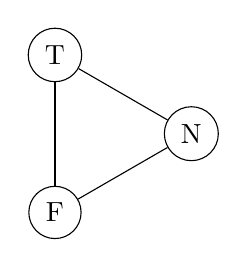
\begin{tikzpicture}
	      \node[shape=circle,draw=black] (A) at (0,0) {F};
	      \node[shape=circle,draw=black] (B) at (0,2) {T};
	      \node[shape=circle,draw=black] (C) at ({sqrt(3)},1) {N};
	      \path [-](A) edge (B);
	      \path [-](A) edge (C);
	      \path [-](B) edge (C);
	\end{tikzpicture}
	\caption{The color palette gadget (T,F,N).}\label{fig:ga:pa}
    \end{subfigure}%
    \begin{subfigure}[t]{0.333\textwidth}
        \centering
	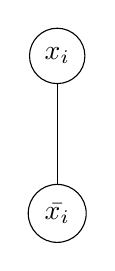
\begin{tikzpicture}
	      \node[shape=circle,draw=black] (A) at (0,2) {$x_i$};
	      \node[shape=circle,draw=black] (B) at (0,0) {$\bar{x_i}$};
	      \path [-](A) edge (B);
	\end{tikzpicture}
	\caption{The variable gadget ($x_i$,$\bar{x_i}$).}\label{fig:ga:va}
    \end{subfigure}%
    \begin{subfigure}[t]{0.333\textwidth}
        \centering
	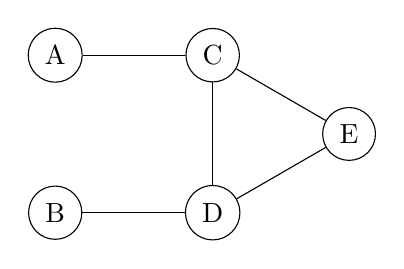
\begin{tikzpicture}
	      \node[shape=circle,draw=black] (A) at (0,2) {A};
	      \node[shape=circle,draw=black] (B) at (0,0) {B};
	      \node[shape=circle,draw=black] (C) at (2,2) {C};
	      \node[shape=circle,draw=black] (D) at (2,0) {D};
	      \node[shape=circle,draw=black] (E) at ({2+sqrt(3)},1) {E};

	      \path [-](A) edge (C);
	      \path [-](B) edge (D);
	      \path [-](C) edge (D);
	      \path [-](C) edge (E);
	      \path [-](D) edge (E);
	\end{tikzpicture}
	\caption{``OR'' gadget (A,B,C,D,E).}\label{fig:ga:or}
    \end{subfigure}
    \caption{Gadgets.}\label{fig:ga}
\end{figure}
The color palette gadget (T,F,N) shown in~\ref{fig:ga:pa} will allow us to give meaning
to the colors of a 3-coloring of our constructed graph.
The variable gadget ($x_i$,$\bar{x_i}$)~\ref{fig:ga:va} and the ``OR'' gadget
(A,B,C,D,E)~\ref{fig:ga:or} will be used to encode $\phi$. To understand where
the ``OR'' gadget gets its name from, let us suppose we want a proper 3-coloring
$(t,f,n)$ of the gadget. In what follows, we will say ``color the
vertex $Z$ with color $x$'' when we mean ``add vertex $Z$ to set $x$''. As is
easily checked, as soon as one of the input vertices A or B of the gadget is
colored with color $t$ we can complete the proper 3-coloring and get E to be
colored with $t$. However, if both input vertices A and B are colored $f$,
there is no way to complete the proper 3-coloring and get E to be colored
with $t$. When thinking about the colors $t$ and $f$ as boolean value true and
false, one sees the similarity between this gadget and the logic ``OR'' gate.

\paragraph{Construction}
\begin{figure}
    \centering
    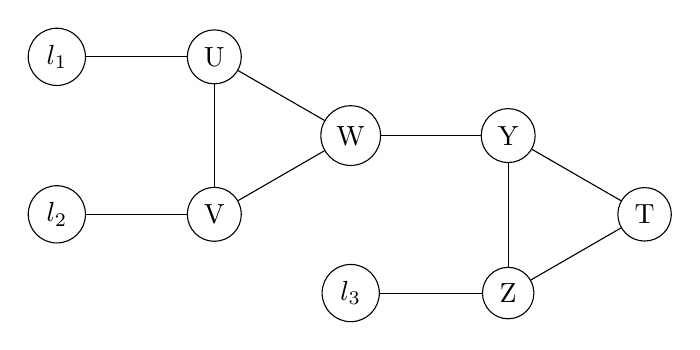
\begin{tikzpicture}
	\node[shape=circle,draw=black] (A) at (0,2) {$l_1$};
	\node[shape=circle,draw=black] (B) at (0,0) {$l_2$};
	\node[shape=circle,draw=black] (C) at (2,2) {U};
	\node[shape=circle,draw=black] (D) at (2,0) {V};
	\node[shape=circle,draw=black] (E) at ({2+sqrt(3)},1) {W};

	\node[shape=circle,draw=black] (BB) at ({2+sqrt(3)},-1) {$l_3$};
	\node[shape=circle,draw=black] (CC) at ({4+sqrt(3)},1) {Y};
	\node[shape=circle,draw=black] (DD) at ({4+sqrt(3)},-1) {Z};
	\node[shape=circle,draw=black] (EE) at ({4+2*sqrt(3)},0) {T};

	\path [-](A) edge (C);
	\path [-](B) edge (D);
	\path [-](C) edge (D);
	\path [-](C) edge (E);
	\path [-](D) edge (E);

	\path [-](E) edge (CC);
	\path [-](BB) edge (DD);
	\path [-](CC) edge (DD);
	\path [-](CC) edge (EE);
	\path [-](DD) edge (EE);
    \end{tikzpicture}
    \caption{The clause gadget.}\label{fig:ga:cl}
\end{figure}
We start with an empty graph. Add a single palette gadget (T,F,N).
For each variable $x_i$ add a single variable gadget ($x_i$,$\bar{x_i}$) and
add an edge from $x_i$ to N and from $\bar{x_i}$ to N.
For each clause $(l_1 \lor l_2 \lor l_3)$ of $\phi$, where
$l_j\in\{\,x_1,\bar{x_1},x_2,\bar{x_2},\ldots,x_n,\bar{x_n}\,\}$,
we add five new vertices U, V, W, Y and Z and connect them to the rest of the
graph with the
two ``OR'' gadgets ($l_1$,$l_2$,U,V,W) and (W,$l_3$,Y,Z,T)
as shown in~\ref{fig:ga:cl}. The complete construction for
$\phi = (x_1 \lor x_2 \lor x_3) \land (\bar{x_1} \lor \bar{x_3} \lor x_4)$
is depicted in~\ref{fig:construction}.
\begin{figure}
    \centering
    \begin{tikzpicture}

	\node[shape=circle,draw=black,fill=white] (T) at (13,-1) {T};
	\node[shape=circle,draw=black,fill=white] (N) at (13,1) {N};
	\node[shape=circle,draw=black,fill=white] (F) at ({13+sqrt(3)},0) {F};
	\begin{pgfonlayer}{bg}
	    \path [-](T) edge (F);
	    \path [-](T) edge (N);
	    \path [-](F) edge (N);
	\end{pgfonlayer}

	\node[shape=circle,draw=black] (x1) at (0,0) {$x_1$};
	\node[shape=circle,draw=black] (x11) at (2,0) {$\bar{x_1}$};
	\begin{pgfonlayer}{bg}
	  \path [-](x1) edge (x11);
	  \draw [-](x1) |- ($(N)+(0,-0.175)$);
	  \draw [-](x11) |- ($(N)+(0,-0.125)$);
	\end{pgfonlayer}

	\node[shape=circle,draw=black] (x2) at (3,0) {$x_2$};
	\node[shape=circle,draw=black] (x22) at (5,0) {$\bar{x_2}$};
	\begin{pgfonlayer}{bg}
	  \path [-](x2) edge (x22);
	  \draw [-](x2) |- ($(N)+(0,-0.075)$);
	  \draw [-](x22) |- ($(N)+(0,-0.025)$);
	\end{pgfonlayer}

	\node[shape=circle,draw=black] (x3) at (6,0) {$x_3$};
	\node[shape=circle,draw=black] (x33) at (8,0) {$\bar{x_3}$};
	\begin{pgfonlayer}{bg}
	  \path [-](x3) edge (x33);
	  \draw [-](x3) |- ($(N)+(0,0.025)$);
	  \draw [-](x33) |- ($(N)+(0,0.075)$);
	\end{pgfonlayer}

	\node[shape=circle,draw=black] (x4) at (9,0) {$x_4$};
	\node[shape=circle,draw=black] (x44) at (11,0) {$\bar{x_4}$};
	\begin{pgfonlayer}{bg}
	  \path [-](x4) edge (x44);
	  \draw [-](x4) |- ($(N)+(0,0.125)$);
	  \draw [-](x44) |- ($(N)+(0,0.175)$);
	\end{pgfonlayer}

	\node[shape=circle,draw=black] (U1) at (3,-9) {$U_1$};
	\node[shape=circle,draw=black] (V1) at (3,-7) {$V_1$};
	\node[shape=circle,draw=black] (W1) at ({3+sqrt(3)},-8) {$W_1$};

	\node[shape=circle,draw=black] (Y1) at (6,-8) {$Y_1$};
	\node[shape=circle,draw=black] (Z1) at (6,-6) {$Z_1$};

	\begin{pgfonlayer}{bg}
	\draw [-](x1) |- (U1);
	\path [-](x2) edge (V1);
	\path [-](U1) edge (V1);
	\path [-](U1) edge (W1);
	\path [-](V1) edge (W1);

	\path [-](W1) edge (Y1);
	\path [-](x3) edge (Z1);
	\path [-](Y1) edge (Z1);
	\draw [-](Y1) -| ($(T)+(0.05,0)$);
	\draw [-](Z1) -| ($(T)+(0.00,0)$);
	\end{pgfonlayer}

	\node[shape=circle,draw=black] (U2) at (8,-4) {$U_2$};
	\node[shape=circle,draw=black] (V2) at (8,-2) {$V_2$};
	\node[shape=circle,draw=black] (W2) at ({8+sqrt(3)},-3) {$W_2$};

	\node[shape=circle,draw=black] (Y2) at (11,-3) {$Y_2$};
	\node[shape=circle,draw=black] (Z2) at (11,-1) {$Z_2$};

	\begin{pgfonlayer}{bg}
	\draw [-](x11) |- (U2);
	\path [-](x33) edge (V2);
	\path [-](U2) edge (V2);
	\path [-](U2) edge (W2);
	\path [-](V2) edge (W2);

	\path [-](W2) edge (Y2);
	\draw [-](x4) |- (Z2);
	\path [-](Y2) edge (Z2);
	\draw [-](Y2) -| ($(T)+(-0.05,0)$);
	\path [-](Z2) edge (T);
	\end{pgfonlayer}
    \end{tikzpicture}
    \caption{The construction of $\langle G \rangle = f(\langle \phi \rangle)$ for
    $\phi = (x_1 \lor x_2 \lor x_3) \land (\bar{x_1} \lor \bar{x_3} \lor x_4)$.}\label{fig:construction}
\end{figure}

Here is a corresponding \emph{Turing-machine-like} description of the algorithm
\begin{TMachine}{$f =$ on input $\langle \phi \rangle$:}
\item[1.] $V \gets \{\,T,F,N\,\}$.
\item[2.] $E \gets \{\,\{\,T,F\,\},\{\,F,N\,\},\{\,N,T\,\}\,\}$.
\item[3.] For each variable $x_i$,
\item[3.1.] $V \gets V \cup \{\,x_i,\bar{x_i}\,\}$.
\item[3.2.] $E \gets E \cup
  \{\,\{\,x_i,\bar{x_i}\,\},\{\,x_i,N\,\},\{\,\bar{x_i},N\,\}\,\}$.
\item[4.] For each clause $c_k = (l_1\lor l_2\lor l_3)$,
\item[4.1.] $V \gets V \cup \{\,U_k,V_k,W_k,Y_k,Z_k\,\}$.
\item[4.2.] $E \gets E \cup \{\,
\{\, l_1 , U_k\,\},
\{\,l_2 , V_k\,\}
  \,\}$.
\item[4.3.] $E \gets E \cup \{\,
\{\,    U_k , V_k\,\},
\{\,  U_k , W_k\,\},
\{\,V_k , W_k\,\}
  \,\}$.
\item[4.4.] $E \gets E \cup \{\,
\{\,    W_k , Y_k\,\},
\{\,  l_3 , Z_k\,\}
  \,\}$.
\item[4.5.] $E \gets E \cup \{\,
\{\,Y_k , Z_k\,\},
\{\,    Y_k , T\,\},
\{\,  Z_k , T\,\}
  \,\}$.
\item[5.] Output $\langle (V,E) \rangle$.
\end{TMachine}

\subsubsection{Complexity}
An important step when reducing an NP-complete problem to an NP problem is to
check that the reduction takes polynomial time and that the new problem is of
polynomial size.

It is not difficult to see that the complexity of the algorithm above is
linear. Let $n$ denote the number of variables of $\phi$ and $m$ denote the
number of its clauses. We have $\card{V} = 3 + 2n + 5m$ and $\card{E} = 3 +
3n + 10m$. Let $\card{\phi} = 3m$, because there are three literals per clause,
and note that $n \le 3m$, because each clause can introduce at most three new
variables. Then, the size of the output graph, $\card{G} = \card{V} + \card{E}$,
is $O(\card{\phi})$. $f$ runs thus in polynomial time (in its input size)
and produces a graph of polynomial size.

\subsubsection{Correctness}

We need to prove that $\langle \phi \rangle \in \text{3SAT} \iff f(\langle \phi \rangle) \in
\text{3-COLORING}$. We prove the two implications of the equivalence.

\paragraph{($\implies$)} If $\langle\phi\rangle \in \text{3SAT}$ then, by definition,
there exists an assignment $(x_1', x_2', \ldots, x_n') \in \{0,1\}^n$ such
that for each clause there is at least one literal $l_{j,z_j}$ that evaluates
to true.
Let $A$, $B$, and $C$ be three empty sets. In what follows, we will say ``color the
vertex $v$ with color $K$'' when we mean ``add vertex $v$ to set $K$''.
%
Color the vertex $T$ with color $A$,
the vertex $F$ with color $B$, and
the vertex $N$ with color $C$.
For each variable $x_i$, if $x_i'=1$, color the vertex $x_i$ with $A$ and
$\bar{x_i}$ with $B$, otherwise, if $x_i'=0$, color the vertex
$x_i$ with $B$ and $\bar{x_i}$ with $A$. This partial 3-coloring is allowed,
because, by construction, the vertices $x_i$ and $\bar{x_i}$ must
have different colors and cannot be colored with $C$. With this partial proper
3-coloring, each clause gadget has at least
one input vertex colored $A$ and, by construction of the clause gadgets,
there is a 3-coloring of the clause gadget with the three input vertex colors
as chosen above, and the color of the output vertex, $T$, set to $A$, as
chosen. Hence $G$ has a proper 3-coloring,
and $f(\langle \phi \rangle) \in \text{3-COLORING}$.

\paragraph{($\impliedby$)} Conversely, if $f(\langle \phi \rangle) = \langle G
\rangle \in \text{3-COLORING}$,
then, by definition, $G$ must have a proper 3-coloring $(A,B,C)$. Without loss
of generality, assume $T\in A, F\in B$, and $N\in C$. Then all vertices $x_i$
and $\bar{x_i}$ must be colored either with $A$ or $B$. Because $T\in A$,
the only way for the 3-coloring to exist is to have, for each clause gadget,
at least one of the input vertices colored with $A$. A satisfying assignement
for $\phi$ has, for each clause of $\phi$, at least one of its literals set
true. Hence, a satisfying assignment $(x_1', x_2', \ldots, x_n')$ is easily
deduced from the proper 3-coloring of $G$: set $x_i'=1$ if the vertex $x_i$ is
colored $A$, otherwise set $x_i'=0$. Hence, $\langle \phi \rangle \in$ 3SAT.

\subsection{About Karp reductions}

What we just did is called a Karp reduction. Given two languages $A$
and $B$, an algorithm for deciding $B$, and a polynomial-time
mapping procedure $f$ such that
$a \in A$ if and only if $f(a) \in B$, we can decide whether $a \in A$ using
the following algorithm
\begin{TMachine}{On input $a$:}
\item[1.] Translate instance $a \in A$ to the corresponding instance $f(a) \in
	B$ in polynomial time.
\item[2.] Answer the same as the algorithm for $B$ run on $f(a)$.
\end{TMachine}
Moreover, if the algorithm for $B$ runs in polynomial time so does this
algorithm.

\subsection{3-COLORING is NP-complete}

Let us recall the definition of NP-completeness
\begin{definition}
	A language $B$ is NP-complete if it satisfies two conditions:
	\begin{enumerate}
		\item $B$ is in NP, and
		\item every $A$ in NP is polynomial-time reducible to $B$.
	\end{enumerate}
\end{definition}

In a previous lecture we have seen that
\begin{theorem}
	CNF-SAT is NP-complete
\end{theorem}
and that
\begin{theorem}
	CNF-SAT $\le_P$ 3SAT.
\end{theorem}
Those two theorems together with the one we just proved and the fact that
3-COLORING is in NP\footnote{Left as exercise for the reader}
imply the following corollary
\begin{corollary}
	3-COLORING is NP-complete.
\end{corollary}
